\section{Degenerazione degli stati}
Per studiare l'occupazione delle bande è necessario sapere quale distribuzione seguono gli elettroni nelle bande stesse. Il punto di partenza che consideriamo noto è la distribuzione di Fermi-Dirac:
\newl{n[E(k)]=\frac{1}{1+e^{\frac{1}{k_BT}(E(k)-\mu)}}}
dove $\mu$ indica il potenziale chimico da cui si deduce l'energia di Fermi come $\mu_{(T=0)}=\varepsilon_F$.
\begin{figure}
	\centering
	\fbox{
		\begin{tikzpicture}[scale=1,auto=center]
			%\draw [help lines] (0,0) grid (2,2);
			\draw [->] (-1,0) -- (5,0);
			\draw [->] (0,-1) -- (0,5);
			\node[] at (-0.7,4.5) {$n[E(k)]$};
			\node[] at (4.5,-0.25) {$E(k)$};
			\node[] at (-0.25,2.5) {$1$};
			\node[] at (2.5,-0.25) {$\mu_{(T=0)}$};
			\draw[] (-0.1,2.5) -- (0.1,2.5);
			\draw[] (0,2.5) -- (2.5,2.5);
			\draw[]	(2.5,2.5) -- (2.5,0);
			\node[] at (2.55,2.75) {$T=0$};
			\draw[blue,domain=0:5] plot (\x,{2.5/(1+ exp((\x-2.5)*2 )) });
			\draw[green,domain=0:5] plot (\x,{2.5/(1+ exp((\x-2.5)*3 )) });
			\node[] at (1,1.5) {$T\neq0$};
		\end{tikzpicture}
	}
	\caption{Distribuzione di Fermi in funzione di $E(k)$ e di $T$.}
	\label{Fermi}
\end{figure}
Come si può notare dalla Fig.\ref{Fermi} la distribuzione degli elettroni, in approssimazione di $T=0$ è una funzione gradino. Tutti i modelli che verranno studiati sono pensati a T=0. Se $f(E)$ è una funzione di distibuzione di una certa quantità, allora è necessario definire cosa si intende con quantità media di una grandezza fisica del sistema in esame. La definiamo come:
\newl{\langle A\rangle = \frac{1}{N}\sum_{stati}A(E)f(E) = \frac{1}{N}\int_0^{+\infty}dE\,g(E)A(E)f(E)}
dove con $g(E)$ si vuole indicare la \textit{degenerazione degli stati} cioè quanti stati sono presenti in un intervallo di energie $[E,E+dE]$. La funzione di degenerazione degli stati varia in funzione al problema. Per esempio per un elettrone libero di muoversi in un box cubico di lato $L$ (considerando $L\to\infty$ in questo modo tutte le somme sono integrali) con condizioni al contorno periodiche di Born-Von Karman, è possibile calcolare in modo esplicito la forma di g(E). Il punto di partenza è la funzione di partizione per un sistema di particelle. 
\newl{Z &=& \sum_{n_x,n_y,n_z} \exp\left[-\beta\frac{\hbar^2}{2m}\left(\frac{2\pi}{L}\right)^2(n_x^2+n_y^2+n_z^2)\right]=\int dn_x\, dn_y\,dn_z...=\\
&=&\int\,dEg(E)f(E) \nonumber}
E il punto è calcolare $g(E)$ che rappresenta il numero degli stati compresi tra $E$ e $E+dE$. Quindi posso definirla come
\newl{g(E)=\frac{dN}{dE}}
Il passaggio da somma ad integrale su tutti i possibili stati è possibile farlo grazie al fatto che $L\to\infty$.
E' stato fatto anche il seguente cambio di variabili passando dall'energia ai $k$ ed infine agli $n$
\newl{E=\frac{\hbar^2}{2m_e}k^2} 
dove i vari vettori $k_i$ vanno considerati con condizioni al bordo periodiche di Born-Von Karman, quindi 
\newl{k_i=\frac{2\pi}{L}n_i \implicaa \Delta n = \frac{L}{2\pi}\Delta k }.
Differenziando e sostituendo nella forma dell'energia per la particella libera ottengo che
\newl{dE = \frac{\hbar^2}{m}k\,dk.}
Ora calcolo l'integrale usando le coordinate sferiche
\newl{N= \int_{-\infty}^{+\infty} dn_x dn_y dn_z = \frac{L^3}{(2\pi)^2}4\pi\int_0^\infty dk\,k^2}
sostituisco con l'energia e ottengo
\newl{\frac{L^3}{(2\pi)^2}4\pi\int_0^\infty dk\,k^2 = \frac{L^3}{(2\pi)^2} \int_0^{\infty} dE\, \frac{m}{\hbar^2}\frac{\sqrt{2mE}}{\hbar} =\int dEg(E)}
quindi posso dire che
\newl{g(E)_{3D}=2_s\frac{V}{4\pi^2}\left(\frac{2m_e}{\hbar^2}\right)^{\frac{3}{2}}\sqrt{E}}
Siamo in approssimazione di $T=0$, quindi se vogliamo sapere il numero di elettroni con una certa energia $E$ l'integrale verrà taglaito all'energia di Fermi
\newl{N=\int_{-\infty}^{+\infty}dE\,g(E)_{3D}E = \int_0^{E_F} dE\,g(E)_{3D}E}
da qui ho la definizione dell'energia di fermi come:
\newl{E_F=\frac{\hbar^2}{2m}\left(3\pi^2\frac{N}{V}\right)^{\frac{3}{2}}}
\subsection{Degenerazione degli stati in una banda}
Nella sezione precedente è stato possibile calcolare la degenerazione degli stati per un modello di particella libera in uno spazio tridimensionale. Cerchiamo di estendere questo ragionamento applicandolo alle bande elettriniche dei solidi trovate in precedenza. Per estendere il concetto ad una banda elettronica partiamo nel definire la sommatoria su tutti gli stati come 
\newl{\sum_{n}\int_0^{+\infty}dEg_n(E)= 2\frac{V}{(2\pi)^3} \sum_n\int_{-\pi/a}^{+\pi/a} dk_x dk_y dk_z}
dove $n$ identifica il \textit{numero di banda}. L'obiettivo che quindi ci si pone è quello di trovare una formula generale per la $g_n(E)$ che indichi la degenerazione degli stati in funzione del numero di banda che compare come parametro, bisogna quindi avere una definizione di degenerazione degli stati per una banda. Per ottenerla si parte sempre dalla definizione generale precedente cioè, \text{numero di stati contenuti in un range di energie da $E$ a $E+\delta E$} con la particolarità di far rientrare in $E$ la struttura a bande. Consideriamo la Fig.~\ref{INTERVAL}
\begin{figure}
	\centering
		\begin{tikzpicture}[scale=3,auto=center]
			\draw [help lines] (0,0) grid (2,2);
			\draw (1,1) circle (0.2);
			\draw (1,1) circle (0.4);
			\draw[->, rotate around={315:(1,1)}](1,1.2) -- (1,1.4);
			\node[] at (1.3,1.1) {$\delta k$};

		\end{tikzpicture}
	\caption{Spazio $k$ con incremento di energia sufficientemente piccolo.}
	\label{INTERVAL}
\end{figure}
prendiamo nello spazio $k$ un'energia $E$ ed identifichiamo le sup. ad energia costante. Si identifichi un incremento $\delta k$ sufficientemente piccolo. A questo punto è possibile identificare la definizione di degenerazione degli stati di una banda, come nel caso 3D di particella libera, la definizione di $g_n(E)$ risulterà essere il numero di stati compresi nella corona circolare con estremi da $E_n$ a $E_n+(\hbar^2/m) k_n \delta k$. Definendo 
\newl{\chi_n(E)=1 \;\;\;\; \text{ se } E<E_n<E_n+dE \;\;\;\;\; \text{ else } \chi_n=0} 
è possibile scrivere la $g_n(E)$
\newl{g_n(E)dE=\frac{V}{(2\pi)^3}\int_{-\pi/a}^{+\pi/a} dk_x dk_y dk_z \chi_n = \frac{V}{(2\pi)^3}\int_{S_n(E)}dS\delta k}
dove $S_n(E)$ rappresenta la superficie della corona circolare. Sono superfici ad energia costante quindi
\newl{dE(k) = \abs{\nabla E_n(k)} \delta k}.
Inserendo tutto nella formula precedente si ottiene la scrittura della degenerazione degli stati nelle bande generalizzata al parametro di banda $n$
\newl{g_n(E)=\frac{V}{(2\pi)^3} \int_{S_n(E)}\frac{dS}{\abs{\nabla E(k)} } .}
\`E d'obbligo far notare che sulla superficie di Brillouin il gradiente dell'energia è nullo, annullando il denominatore dell'integranda. E' possibile comunque dimostrare che in 2D e in 3D l'integrale continua a convergere.
\subsection{Singolarità di Van Hove e regola d'oro di Fermi}
Riprendendo la forma delle degenerazione degli stati per una banda in un cristallo 
\newl{g_n(E) = \frac{V}{(2\pi)^3} \int_{S_n(E)}\frac{dS}{\abs{\nabla E(k)} } }
come da nota precedente è opportuno discutere il senso di questo integrale per zone vicine alle superficie della prima zona di Brillouin. Le superfici di energia costante intersecano in modo otogonale la superficie di Brillouin avendo, in quei punti, la condizione $\nabla E(k_{Brillouin}) =0$. I punti che soddisfano questa condizione sono chiamati punti di \textit{\textbf{singolarità di Van Hove.}} In questi punti il denominatore dell'integrale si annulla rendendo quindi obbligatoria una discussione della sua convergenza. Come è stato già detto precedentemente, si può dimostrare che in 2 e 3 dimensioni l'integrale continua a convergere. Direttamente collegato alla degenerazione degli stati è lo spettro di assorbimento otticodel cristallo. La probabilità di emissione è data dalla nota regola d'oro di Fermi
\newl{W_{if} = \frac{2\pi}{\hbar}\abs{\bra{i} H \ket{f} } ^2 \rho(\hbar\omega_{if} -\hbar\omega) }
dove con $i-f$ si intendono lo stato di inizio $(i)$ e lo stato di fine $(f)$ e con $W_{if}$ la probabilità di passare da uno all'altro. \`E presente anche una densità $\rho$ che idnetifica il numero di stati. Quindi la probabilità di fare emissione sarà in un qualche modo collegata alla densità di elettroni nella banda a quella determinata energia $\hbar\omega$. Se ne deduce che essendo le singolarità di Van Hove punti di divergenza dell'integrale, quindi punti in cui la funzione $g_n(E)$ è molto piccata, in quei punti è molto più favorita l'emissione di elettroni. Da notare come i punti di singolarità siano in prossimità dei punti di diffrazione idetificati nella teoria di Von Laue. L'elettrone arriva in quella zona di singolarità, particolarmente critico che ha una buona possibilità di essere emesso o difratto.

\begin{center}
\fbox{
\begin{tikzpicture}[scale=1,auto=center]
	\draw[->] (-1,0) -- (5,0);
	\draw[->] (0,-1) -- (0,5);
	\node[] at (5,-0.25) {$E$};
	\node[] at (-0.55,5) {$g_n(E)$};
	\draw (1,0) parabola bend (1,0) (3, 0.3*3^2);
	\draw (3, 0.3*3^2) parabola bend (3, 0.3*3^2) (4.5, 0);
	\node[fill,thick,circle, inner sep=0pt, minimum size=0.2cm] at (3,0.3*3^2)  {};
	\node[] at (3,0.3*3^2+0.25) {$\text{Singolarità di VH}$};
\end{tikzpicture}
}
\end{center}

\subsection{Esempi di elettrone vincolato}
Nella sezione precedente è stato possibile ricavare una forma generale per il calcolo della degenerazione delle bande. Di seguito si applicherà il concetto a diversi tipi di modelli quali \textit{quantum dot} e \textit{quantum well}.
\subsubsection{Quantum dot}
Il quntum dot, meglio conosciuto come atomo artificiale, è rappresentato da un sistema in cui gli elettroni sono vincolati in dimensioni molto piccole. La condizione di "zero dimensionalità" viene in un qualche modo suggerita dalla trasformata di Fourier e quindi dal principio di indeterminazione di Heisenberg. Se il lato del quantum dot, approssimato ad un cubettino molto piccolo, è $L$ questa sarà la nostra restrizione dimensionale $\Delta x$ a cui sarà associato un limite superiore di $\Delta p \sim \hbar/L$. Basandoci su questioni puramente morali possiamo scrivere il momento dell'elettrone come 
\newl{p\sim \frac{\hbar}{2L}}
considerando in questo modo anche la parte negativa di momento. L'energia dell'elettrone sarà quindi
\newl{E=\frac{p^2}{2m} = \frac{\hbar^2}{8mL^2}.}
Le dimensioni tipiche di un quantum dot sono nell'ordine di $L=10\text{nm}$. Usando $m_e$ risulta un'energia dell'elettrone di $E=0,1\text{eV}$. In realtà si utilizza la massa efficacie che fa risultare l'energia nell'ordine di $E\sim 10 \text{eV}$. Il problema si risolve sempre passando dal problema agli autovalori dell'equazione di Schroedinger risolta con condizioni al bordo di buca di potenziale. Già ora è possibile intuire che avendo delle condizione al bordo di tipo buca di potenziale lo spettro delle energie sarà molto diverso da quallo visto fino ad ora per elettrone libero con condizione al bordo periodiche di Born-Von Karman. Il fatto di avere delle condizioni di buca, potrebbe suggerire il fatto di avere un ground-state, che nei casi precedentemente visti non era presente. L'energia dell'ettone è possibile scriverla come
\newl{E_{n_x,n_y,n_z} = \frac{\hbar^2}{2m}(k_x^2+k_y^2+k_z^2)} 
dove i livelli sono discreti e separati da gap di energie nell'ordine dell'$eV$. C'è degenerazione, lo si nota anche semplicemente osservando che $E_{100} = E_{001}$. Quindi è necessario calcolare $g_{0D}(E)$. In questo caso è molto semplice, dato che le energie sono discrete sarà la somma dell'indice di degenerazione di ogni energia, che indichiamo con $g_j(E_j)$, per una delta di Dirac centrata sul valore dell'energia. Riassumendo il tutto
\newl{g_{0D}(E) = 2_s \sum_j g_j(E_j) \delta(E-E_j).}
\subsubsection{Filo quantico}
Il filo quantico è un altro modello utilizzato nella realtà per cui vale la pena valutare la degenerazione degli stati. \`E caratterizzato da $L_x \gg L_y,L_z$, quindi il problema si risolve  separandolo in due parti. Nella direzione $x$ l'elettrone è libero di muoversi, quindi in $x$ le condizioni al contorno, per il problema agli autovalori, saranno di tipo elettrone libero. Nelle direzione $y,z$ si ha invece confinamento, quindi le condizioni al contorno della funzione d'onda saranno diverse.
\begin{figure}
	\centering
	\fbox{
		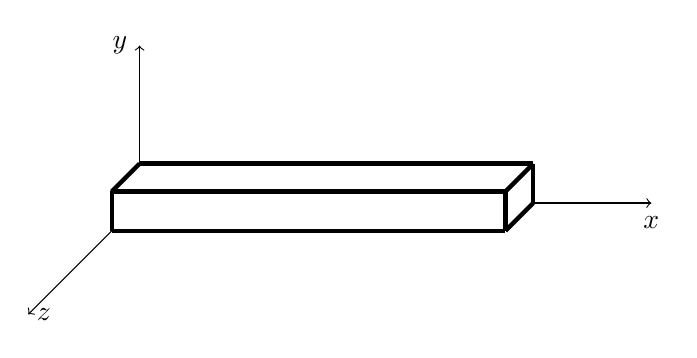
\begin{tikzpicture}[scale=1,auto=center]
			\draw[->] (0,0.5) -- (0,2);
			\draw[->] (5,0) -- (6.5,0);
			\draw[->] (-0.35355,-0.35355) -- (-1.414,-1.414);
			\node[] at (-0.25,2) {$y$};
			\node[] at (6.5,-0.25) {$x$};
			\node[]	at (-1.214,-1.414)   {$z$};
			\draw[ultra thick] (-0.35355,-0.35355) -- (-0.35355,0.146466);
			\draw[ultra thick] (-0.35355,0.146466) -- (0,0.5);
			\draw[ultra thick] (0,0.5) -- (5,0.5);
			\draw[ultra thick] (-0.35355,-0.35355) -- (4.64645,-0.35355);
			\draw[ultra thick] (-0.35355,0.146466) -- (4.64645,0.146466);
			\draw[ultra thick] (4.64645,0.146466) -- (5,0.5);
			\draw[ultra thick] (4.64645,-0.35355) -- (4.64645,0.146466);
			\draw[ultra thick] (4.64645,-0.35355) -- (5,0);
			\draw[ultra thick] (5,0) -- (5,0.5);
		\end{tikzpicture}
	}
	\caption{Modello di filo quantico}
	\label{FILO:Q}
\end{figure}
Facendo riferimento alla Fig.~\ref{FILO:Q} possimao scrivere l'energia del sistema come
\newl{E = E_x + E_\perp = \frac{\hbar^2 k_x^2}{2m} + E(n_y, n_z).}
in $x$ ho la condizione di elettrone libero quindi le condizioni al contorno sono quelle di Born-Von Karman $k_x = n_x 2\pi/L_x$. Su $y$ e $z$ dato che ho confinamento le condizioni al contorno per la funzione d'onda rimarrano quelle di buca. Quindi il problema in questo modo si separa in due parti, su $y$ e $z$ la degenerazione degli stati rimande uguale al quantum dot
\newl{\boxed{g_{y,z}(E_\perp) = \sum_j g_j(E_j)\delta(E_\perp - E_j).}}
Sull'asse $x$ ho libertà quindi ottengo che
\newl{\sum_j \to  \frac{L_x}{2\pi} \int_{-\infty}^{+\infty} dk_x = \frac{L_x}{2\pi} \int_0^{+\infty} dk_x =\frac{L_x}{\pi}\int_0^{+\infty}dE\sqrt{\frac{m}{2E\hbar^2}}}
ottenendo quindi
\newl{g_x(E_x)=\frac{L_x}{\pi} \sqrt{\frac{m}{2\hbar^2}}\frac{1}{\sqrt{E}}.}
Unendo i risultati per ottenere una forma generale di densità degli stati si ottiene
\newl{g_{1D}(E)=\int_{0}^{+\infty}dE_x \int_{0}^{+\infty} dE_\perp g_x(E_x)g_{y,z}(E_\perp)\delta(E-E_x-E_\perp)}
Una cosa che non si capisce bene è la condizione per cui $\int dE_x \neq 0 \to E-E_\perp\geq0$. Con questa condizione definisco una funzione $\theta$ e posso elimanre l'integrale in $x$
\newl{g_{1D}(E)=\frac{L_x}{\pi}\sqrt{\frac{m}{2\hbar^2}} \sum_j g_j(E_j)\int_0^{+\infty} dE_\perp \frac{\delta(E_\perp-E_j)}{\sqrt{E-E_\perp}}\theta(E-E_\perp)} 
ma l'integrale è molto semplice e diventa quindi
\newl{g_{1D}(E)=2_s\frac{L_x}{\pi}\sqrt{\frac{m}{2\hbar^2}} \sum_j g_j(E_j)\frac{\theta(E_\perp-E_j)}{\sqrt{E-E_\perp}}.}
Lo stesso ragionamento lo si può estendere in modo molto semplice anche al caso di un sistema di "piano quantico". In questo caso il confinamento è solo su di un asse mentre sugli altri due ho la condizione di elettrone libero. La forma della degenerazione degli stati discende direttamente da quella del filo quantico
\newl{g_{2D}(E)=2_s\frac{L_xL_y}{2\pi}\frac{m}{\hbar^2}\sum_j\theta(E-E_j)}
\begin{figure}
	\centering
	\fbox{
		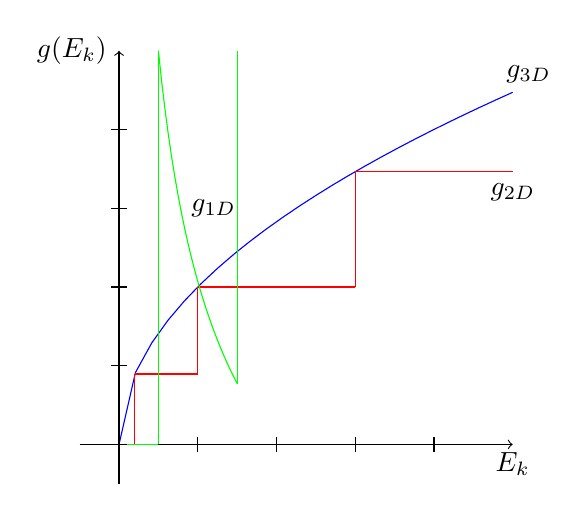
\begin{tikzpicture}[scale=1,auto=center]
			\draw[->] (0,-0.5) -- (0,5);
			\draw[->] (-0.5,0) -- (5,0);
			\node[] at (5.2,4.7) {$g_{3D}$};
			\node[] at (-0.6,5) {$g(E_k)$};
			\node[] at (5,-0.25) {$E_k$};
			%g_3D -> sqrt(E)
			\draw[blue,domain=0:5] plot (\x,{2*sqrt(\x)});
			%g_2D -> Cost.
			\draw[red] (0.2,0) -- (0.2,2*0.44721359549995793928);
			\draw[red] (0.2,2*0.44721359549995793928) -- (1,2*0.44721359549995793928);
			\draw[red] (1,2*0.44721359549995793928) --(1,2);
			\draw[red] (1,2) -- (3,2);
			\draw[red] (3,2) -- (3,2*1.732);
			\draw[red] (3,2*1.732) -- (5,2*1.732);
			%g_1D -> e^{1/2}
			\draw[green] (0,0) -- (0.5,0);
			\draw[green] (0.5,0) -- (0.5,5);
			\draw[green, domain=0.5:1.5] plot (\x,{7.071/sqrt(\x)-5}); 
			\draw[green] (1.5,{7.071/sqrt(1.5)-5}) -- (1.5,5);
			\node[] at (5,3.2) {$g_{2D}$};
			\node[] at (1.2,3) {$g_{1D}$};
			\foreach \p in {0,1,2,3,4} {
				\draw (\p,-0.1) -- (\p,0.1);
				\draw (-0.1,\p) -- (0.1,\p);
			}

		\end{tikzpicture}
	}
	\caption{Degenerazione degli stai per varie dimensioni. \`E ben visibile il comportamento della $g_{3D}\sim\sqrt{E}$ della $g_{2D}\sim\text{cost.}$ e della $g_{1D}\sim1/\sqrt{E}$. Per quando riguarda la $g_{0D}$ è banale perchè è costituita da una serie di delta centrate sulle energie degeneri.}
	\label{DEG:ST}
\end{figure}

